We are interested in {\em holomorphic} superfunctions, so the idea is
not far to consider the Cauchy integral formula:
\begin{wellknown}[Cauchy integral formula]\label{wk:cauchy_integral}
  If $f$ is holomorphic on $D$ and if $A$ is an open disk
  or rectangle such that $A\cup \partial A\subset D$, then 
  \begin{align}\label{eq:cif}
    f(z)=\frac{1}{2\pi \I}\int_{\partial A} \frac{f(\zeta)}{\zeta - z}
    d\zeta
  \end{align}
  for each $z\in A$. And vice versa if $f$ is continuous on $\partial
  A$ then the function
  \begin{align*}
    F(z):=\frac{1}{2\pi \I}\int_{\partial A} \frac{f(\zeta)}{\zeta-z} d\zeta
  \end{align*}
  defined on the interior of $\partial A$ is holomorphic.
\end{wellknown}
Let $\gamma_|$ be a vertical (long though finite) line through a fixed
$x_0\in\R$.
If we choose the left boundary of the rectangle $A$ to be
$\gamma_L=\gamma_|-1$ and the right boundary to be $\gamma_|+1$ and if
we compute the values on $\gamma_|$ by the Cauchy integral formula
then we can recover the values on $\gamma_R$ and $\gamma_L$ by
$\sigma(z+1)=f(\sigma(z))$ and $\sigma(z-1)=f^{-1}(\sigma(z))$.

For the values on the top and bottom boundary $\gamma_T$ and
$\gamma_B$ of $A$ we consider the following. The Abel function (i.e.\
the inverse of $\sigma$) is supposed to have a singularity at a
(chosen) fixed point. In the case of a real analytic function with a
non-real fixed point $z_1$ there must also be a singularity on the
conjugated fixed point $z_{-1}$. This means it would make sense to impose 
 $\lim_{y\to\pm\infty}\sigma(x+\I y)= z_{\pm 1}$ for $x\in (-1,1)$.

So for the rectangle $A$ being tall enough one could just approximate
the values on $\gamma_T$ and $\gamma_B$ by $z_1$ and $z_{-1}$
respectively.

In formulas, we first define the parts of the boundary such that the
concatenation of the parts is a counterclockwise closed path.
\begin{align*}
  &&\gamma_{T,h}(t)&=x_0-t+\I h&&\\
  \gamma_L(t)&=x_0-1-\I t &\gamma_|(t)&=x_0+\I t& \gamma_R(t)&=x_0+1+\I t\\
  &&\gamma_{B,h}(t)&=x_0+t-\I h&&
\end{align*}
The Cauchy integrals of $\sigma$ along $\gamma_L$ and $\gamma_R$ for
$z=\I y$ ($z\in\gamma_|$) are 
\begin{align*}
  \int_{\gamma_R}\frac{\sigma(\zeta)}{\zeta-(x_0+\I y)}\di\zeta 
   &= +\I\int_{-h}^h \frac{\sigma(x_0+1+\I t)}{1+\I t- \I y} \di t
   = \I\int_{-h}^h \frac{f(\sigma(x_0+\I t))}{1+\I (t-y)} \di t
  \\\int_{\gamma_L}\frac{\sigma(\zeta)}{\zeta-(x_0+\I y)}\di\zeta 
   &=-\I\int_{-h}^h \frac{\sigma(x_0-1-\I t)}{-1-\I t -\I y} \di t
   =\I\int_{-h}^h \frac{f^{-1}(\sigma(x_0-\I t))}{1+\I (t+y)} \di t.
\end{align*}
For the top and bottom boundary:
\begin{align*}
    \lim_{h\to\infty}\int_{\gamma_{T,h}}\frac{\sigma(\zeta)}{\zeta-(x_0+\I
      y)}\di\zeta
   &= \lim_{h\to\infty} -z_1\int_{-1}^{1}\frac{\di t}{-t+\I (h -
       y)}
   = \lim_{h\to\infty} z_1\underbrace{\int_{-1}^{1}\frac{\di t}{t-\I (h -
       y)}}_{\lambda(h-y)}
  \\\lim_{h\to\infty}\int_{\gamma_{B,h}}\frac{\sigma(\zeta)}{\zeta-(x_0+\I
    y)}\di\zeta
   &= \lim_{h\to\infty}z_{-1}\int_{-1}^{1}\frac{\di t}{t-\I (h + y)}
    = \lim_{h\to\infty} z_{-1}\lambda(h+y)
  \\\lambda(d) &= \log(1-\I d) - \log(-1-\I d) =
  2\I\left(\frac{\pi}{2}-\arctan(d)\right), \quad d>0
\end{align*}
We put them together with the Cauchy integral formula \ref{eq:cif}
to obtain a recurrence
\begin{align*}
\sigma(x_0+\I y)&=\lim_{h\to\infty}\frac{1}{2\pi} \int_{-h}^h\left(
   \frac{f(\sigma(x_0+\I t))}{1+\I (t- y)}
   +\frac{f^{-1}(\sigma(x_0-\I t))}{1+\I (t+ y)}
   \right)\di t + \frac{z_1\lambda(h-y) +
     z_{-1}\lambda(h+y)}{2\pi \I}
\end{align*}
This roughly describes the iteration process we use. We approximate
$h\to\infty$ by a big enough number and establish a grid on $\gamma_|$
of $\sigma$ values. The integration is carried out numerically.

Without changing the obtained $\sigma(x_0+\I y)$ we can replace $x_0$ by any other
number, particularly $x_0=0$.

It is however not yet proven (for $f(x)=e^x$ and any other function) that this
iteration process indeed converges. Not even that if it converges then
the resulting function is a holomorphic superfunction. On the other
hand the numerical results support all these 3 claims ((1.)convergence  to
a (2.)holomorphic (3.)superfunction).


% However if it converges, the resulting $\sigma$ is holomorphic as well as a superfunction.
% \begin{proposition}
%   Let $\sigma$ be a continuous function defined on $x_0+\I \R$ for
%   some $x_0\in\R$. Let $f$ be an injective holomorphism on
%   $\sigma(x_0+\I \R)$ with fixed points $z_1$ and $z_{-1}$ such that
%   $\lim_{y\to\infty} \sigma(x+\I y)=z_{\pm 1}$. If $\sigma$ satisfies
%   \begin{align}\label{eq:Kouznetsov_integral}
%     \sigma(x_0+\I y)&=\lim_{h\to\infty}\frac{1}{2\pi} \int_{-h}^h\left(
%    \frac{f(\sigma(x_0+\I t))}{-(x_0-1)+\I (t- y)}
%    +\frac{f^{-1}(\sigma(x_0+\I t))}{-(x_0+1)+\I (t- y)}
%    \right)\di t
%   \end{align}
%   then $\sigma$ is a holomorphic superfunction of $f$ continuable to all $z$ with
%   $\Re(z)>-1$.
% \end{proposition}
% \begin{proof}
%   First we define $\sigma(x_0\pm 1+\I t):=f^{\pm 1}(\sigma(x_0+\I t))$ and
%   notice that $\sigma$ is a continuous function on the on the Riemann
%   sphere closed Jordan curve $x_0+1+\I[-\infty,\infty]\cup
%   x_0-1+\I[-\infty,\infty]$. As the limit in
%   \eqref{eq:Kouznetsov_integral} exists, we know that $\sigma$ is a
%   holomorphic function on $\I\R$ continueable to $(x_0-1,x_0+1)+\I\R$.
% \end{proof}


\subsection{Application to the exponential}
This function is shown in figure
\ref{figsexpG}.
\begin{figure}
\begin{center}
\sx{2.4}{\begin{picture}(320,110)
%\put(0,0){\includegraphics{../cauchi/figsexpG}}
%\put(0,0){\includegraphics{cauchi/figsexpG}}
\put(-10,0){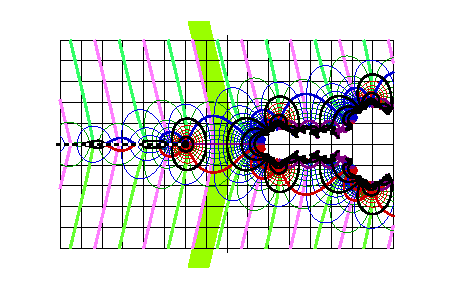
\includegraphics{cauchi/figvladi02a}}
\put(  1,111){\sx{.6}{$\Im(z)$}}
\put(  7, 99){\sx{.58}{$4$}}
\put(  7, 89){\sx{.58}{$3$}}
\put(  7, 79){\sx{.58}{$2$}}
\put(  7, 69){\sx{.58}{$1$}}
\put(  7, 59){\sx{.58}{$0$}}
\put(  2, 49){\sx{.58}{$-1$}}
\put(  2, 39){\sx{.58}{$-3$}}
\put(  2, 29){\sx{.58}{$-3$}}
\put(  2, 19){\sx{.58}{$-4$}}
\put(  2,  9){\sx{.58}{$-5$}}
\put(170,4){\sx{.6}{$\Re(z)$}}
\put(150,4){\sx{.6}{$6$}}
\put(130,4){\sx{.6}{$4$}}
\put(110,4){\sx{.6}{$2$}}
\put( 90,4){\sx{.6}{$0$}}
\put( 66,4){\sx{.6}{$-2$}}
\put( 46,4){\sx{.6}{$-4$}}
\put( 26,4){\sx{.6}{$-6$}}
%\put(12,115){\rot{-70}{\sx{.6}{$\Im(f)\!=\!L$}}\ero }
\put( 38,115){\rot{-77}{\sx{.4}{$\Im(f)\!=\!\Im(L)$}}\ero }
\put( 50,115){\rot{-77}{\sx{.4}{$\Re(f)\!=\!\Re(L)$}}\ero }
\put( 62,115){\rot{-77}{\sx{.4}{$\Im(f)\!=\!\Im(L)$}}\ero }
\put( 98,115){\rot{-77}{\sx{.4}{$\Re(f)\!=\!\Re(L)$}}\ero }
\put(108,115){\rot{-77}{\sx{.4}{$\Im(f)\!=\!\Im(L)$}}\ero }
\put(120,115){\rot{-77}{\sx{.4}{$\Re(f)\!=\!\Re(L)$}}\ero }

\put( 42,14){\rot{77}{\sx{.4}{$\Im(f)\!=\!-\!\Im(L)$}}\ero }
\put( 53,14){\rot{77}{\sx{.4}{$\Re(f)\!=\!\Re(L)$}}\ero }
\put( 65,14){\rot{77}{\sx{.4}{$\Im(f)\!=\!-\!\Im(L)$}}\ero }

\put( 81, 8){\rot{ 76.7}{\sx{.66}{$\mathrm{arctet}(G)$}}\ero }
\end{picture}}

\sx{2.4}{\begin{picture}(320,125)
%\put(0,0){\includegraphics{../cauchi/figslogG}}
%\put(0,0){\includegraphics{cauchi/figslogG}}
\put(-10,0){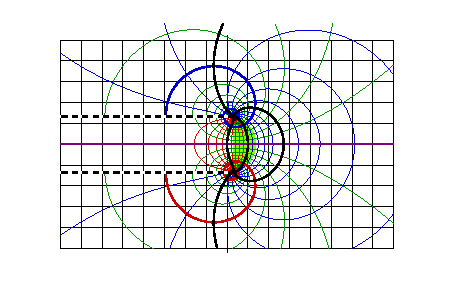
\includegraphics{cauchi/figvladi02b}}
\put( 1,112){\sx{.6}{$\Im(z)$}}
\put( 7, 99){\sx{.58}{$4$}}
\put( 7, 89){\sx{.58}{$3$}}
\put( 7, 79){\sx{.58}{$2$}}
\put( 7, 69){\sx{.58}{$1$}}
\put( 7, 59){\sx{.58}{$0$}}
\put( 2, 49){\sx{.58}{$-1$}}
\put( 2, 39){\sx{.58}{$-2$}}
\put( 2, 29){\sx{.58}{$-3$}}
\put( 2, 19){\sx{.58}{$-4$}}
\put( 2,  9){\sx{.58}{$-5$}}

\put(170,4){\sx{.6}{$\Re(z)$}}
\put(150,4){\sx{.6}{$6$}}
\put(130,4){\sx{.6}{$4$}}
\put(110,4){\sx{.6}{$2$}}
\put( 90,4){\sx{.6}{$0$}}
\put( 66,4){\sx{.6}{$-2$}}
\put( 46,4){\sx{.6}{$-4$}}
\put( 26,4){\sx{.6}{$-6$}}
\put( 95,57){\sx{1}{$G$}}

\put( 46,120){\sx{.4}{$\Re(f)\!=\!2.2$}}
\put( 80,120){\sx{.4}{$\Re(f)\!=\!2$}}
\put(106,120){\sx{.4}{$\Im(f)\!=\!0.6$}}
\put(136,120){\sx{.4}{$\Im(f)\!=\!0.4$}}
\put(171,100){\sx{.4}{$\Im(f)\!=\!0.2$}}
\put(171, 92){\sx{.4}{$\Re(f)\!=\!1.8$}}
\put(172, 60){\sx{.4}{$\Im(f)\!=\!0$}}
\end{picture}}
\end{center}
\caption{functions $f=\mathrm{tet}(z)$ and $f=\mathrm{arctet}(z)$ in the complex 
$z$-plane. \label{figsexpG} }
\end{figure}

% %\newcommand \JP {{}}
% \newcommand \ve {\varepsilon}
% %\subsection{Asymptotics of cauchi-tetration at large imaginary part of the argument}
% \subsection{Expansion of the Cauchy-tetrational at fixed point $L$}
% FOr simplicity, here we consider the only case of base $b=\mathrm e$.
% Asymptotically, the cauchy-tetrational $F$ can be written as follows:
% \begin{align}
% F(z)=\Phi_0(\ve)+
% %\sum_{m=0}^M \beta_n \ve \exp(2 \pi \mathrm{i} m z) \Phi_m(\ve)
% %+\mathcal{O}\!\Big(\ve \exp\big( 2 \pi \mathrm{i} (M+1) z\big) \Big)
% \beta_1 \ve \exp(2 \pi \mathrm{i} z) \Phi_1(\ve)
% +\mathcal{O}\!\Big(\ve^2 \exp\big( 4 \pi \mathrm{i} z\big) \Big)
% \label{eq:dima01}
% \end{align}
% where 
% $\ve=\exp(Lz+R)$
% ~,~ parameters $R$ and $\beta_1$ are complex numbers, and $\Phi_0$, $\Phi_1$ are 
% holomorphic functions, expandable in powerseries 
% \begin{align}
% \Phi_m(x)=\sum_{n=0}^N a_{m,n} x^n + \mathcal{O} \Big( x^{N+1} \Big);
% \end{align}
% $a_{0,0}=L$; 
% $a_{0,1}=1$;
% $a_{1,0}=1$;
% %At $\mathrm i \infty $, $F$ should be $L$, so, $a_{0,0}=L$.
% The substitution of (\ref{eq:dima01}) into equation $F(z+1)=\exp(F(z))$
% and the asymptotical expansion at $|\ve|\ll 1$ determines the coefficients $a$.
% The calculation with Mathematica gives
% \begin{align}
% %a_{0,0}&=L\\
% %a_{0,1}&=1\\
% a_{0,2}&=\frac{1/2}{L-1}\\
% a_{0,3}&=\frac{L+2}{6(L-1)^2(L+1)}\\
% a_{0,4}&=\frac{6+6L+5L^5+L^3}{24(L-1)^3(1+L)(1+L+L^2)}\\
% a_{0,5}&=\frac{24+36L+46L^2+40L^3+24L^4+9L^5+L^6}{120(L-1)^4(1+L)^2(1+L+2L^2+L^3+L^4)}\\
% a_{0,6}&=\frac{\!120\!+\!240L+390L^2+480L^4+416L^5+301L^6+160L^7+64L^8+14L^9+L^{10}}
% {720(L-1)^2(1+L^2)(1+L^2)(1+L+L^2)(1+L+L^2+L^3+L^4)}\\
% %a_{1,0}&=1\\
% a_{1,1}&=%\frac{1}{L-1} = 
% 2 a_{0,2}\\
% a_{1,2}&=%\frac{1+L/2}{(L-1)^2(L+1)} =
% 3 a_{0,3}\\
% a_{1,3}&=%\frac{6+6L+5L^5+L^3}{6(L-1)^3(L+1)(L^2+L+1)} = 
% 4 a_{0,4}\\
% a_{1,4}&=%\frac{24+36L+46L^2+40L^3+24L^4+9L^5+L^6}
% %{24(L-1)^2(1+L)^2(1+L+2L^2+L^3+L^4)} = 
% 5 a_{0,5}\\
% a_{1,5}&=%\frac{\!120\!+\!240L+390L^2+480L^4+416L^5+301L^6+160L^7+64L^8+14L^9+L^{10}}
% %{120(L-1)^2(1+L^2)(1+L^2)(1+L+L^2)(1+L+L^2+L^3+L^4)}=
% 6 a_{0,6}
% \end{align}

% The tetration equation by itself does not determine the parameter $R$ and 
% coefficints $\beta$. The order of magintude of constant $R$ can be 
% estimated even without a computer, just from the {\em assumption}
% that
% \begin{align}
% \mathrm{tet}(z)\approx 1+\mathrm{tet}'(z)\approx Lz+\exp(Lz+R)
% \label{appro1}
% \end{align}
% and $\mathrm{tet}'(0)\approx 1$; although the more precise estimate 
% gives $\mathrm{tet}'(0)\approx 1.091767351258322138$~.
% Then, the rough estimate for $R$ can be written as follows:
% \begin{align}
% R\approx \ln(1+z)-Lz
% \label{appro2}
% \end{align}

% For $z=i/2$, this gives 
% \begin{align}
% R
% \approx -L \mathrm{i}/2 + \ln(1+\mathrm{i}/2-L)
% \approx 0.745-1.046 \mathrm{i}
% \label{R2}
% \end{align}
% and for $z=i$, we get the estiamte 
% \begin{align}
% R\approx -L \mathrm{i} + \ln(1+\mathrm{i}-L)\approx 1.064-0.777 
% \mathrm{i}
% \label{R1}
% \end{align}
% Similar estimates can be obtained for $z=0$ and $z=-1/2$.
% Comparing \rf{R2} and \rf{R1}, we may {\em expect} that $R\approx 
% 1\!-\!i~$. 
% The second decimal digit in this estimate is already doubtful, and 
% we cannot guess even a first digit of the coefficient $\beta_1$ with 
% such a physically-brutal treate.
% With better precision, the coefficients $R$ 
% and $\beta_1$ can be 
% evaluated, fitting the 
% Cauchy-tetration; this gives values
% \begin{align}
% R &\approx 1.077961437528 -0.9465409639478 ~\mathrm{i}& \\
% \beta_1&\approx ~ 0.12233177 ~ -0.02366104 ~\mathrm{i} &	
% %\\	\beta_2&\approx ~~ - 0.25 ~~ - ~ 0.27 ~\mathrm{i} &\\
% \end{align}
% We believe, these values approximate the fundamental mathematical constants.

% Local Variables:
% TeX-master: "../main"
% End:
